\section{Current method of ULTRACAM data reduction}

Tom Marsh at the University of Warwick has developed a set of software tools that allow the observer to reduce the data for ULTRACAM. For the rest of this document we will refer to this pipeline as the \emph{traditional} pipeline and the new pipeline created in this project as the \emph{automated} pipeline. 

It is possible to run the traditional pipeline at the telescope during the observation. This allows observers to review the data in 'real-time'. This serves as a `preview' for the observer and allows adjustments to be made during the run. After the run, the raw data is copied to the archive and this can be used for reductions later. This can happen the following day, or much later when the observer has returned from the telescope site. This data archive can be `re-reduced' at any time as all of the raw data is stored in the archive. 

The current data reduction process for ULTRACAM is designed to produce three colour light curves from the raw image data. The pipeline consists of the following stages:
\begin{enumerate}
	\item Producing \emph{bias} frames that are used the calibrate the CCD detector's thermal noise characteristics. 
	\item Producing \emph{flat-fields} to calibrate the pixel sensitivity of each of the 3 CCD detectors. These flat-fields are subtracted from the image data during the reduction process.
	\item Defining \emph{apertures} for the objects of interest in the run. This step involves manually choosing the objects of interest in the frames and defining the aperture sizes and positions for each object. Apertures are independently set for each channel (r, g, b). 
	\item Running the \emph{reduction} software. The reduction code uses the apertures defined in the previous step and measures the flux of each object in each colour. The software is able to track changes in the object's size and shape due to changes in the point spread function (PSF) by scaling the virtual aperture. It is also able to track small deviations in the positions of the objects. 
\end{enumerate} 
Although this process is not particularly cumbersome, it \emph{does} include some manual steps and it does not scale well when there are a large number of runs to be processed or if there are many target objects in a run. For example, the run shown in Fig. \ref{fig:KOI-824} contains more than 1000 objects. Manually defining apertures for each of these objects in each channel is not really practical. An automated method enables data reduction for all of the objects captured in each run without the need for manual intervention. 

\subsection{Aperture selection}

\begin{figure}[!h]
\centering
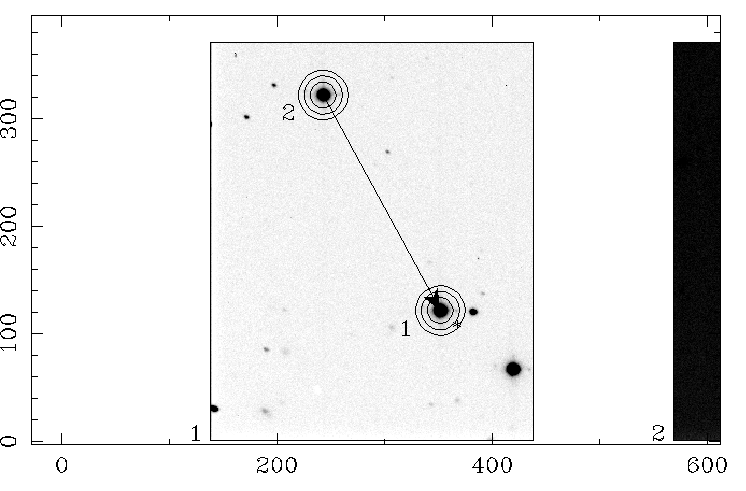
\includegraphics[width=80mm]{images/setaper.png}
\caption{Defining the apertures for the reduction using the \emph{traditional} pipeline. Note that the two apertures can be linked. This instructs the pipeline to maintain the pixel separation of the apertures even if there is a small amount of movement from frame to frame. This is useful if our target object is likely to alter in brightness during the run. }
\label{fig:nnsercomparisontom}
\end{figure}


\subsection{Flat fields and biases}

\subsection{Photometric calibration}

\section{Automating the pipeline}

The outcome of this MSc project is a system that is able to process the raw image data from ULTRACAM and, without any manual intervention, produce a set of light curves for all of the objects in that data. It produces a set of web pages that can be viewed from anywhere with an Internet connection. 

\subsection{Motivation for automating the pipeline}
ULTRACAM has recorded a large amount of photometric data at some of the world's best sites and largest telescopes. Since the CCD captures more objects than the observer is strictly interested in, there is a good chance that some objects of astronomical interest have been captured by ULTRACAM, but not been noticed or analysed during the reduction process. By automating the reduction pipeline we can produce photometry, in other words, 'light curves' for \emph{all} of the objects captured by ULTRACAM and then search through the archive to find new objects of interest. 

An automated pipeline can be run on the data immediately after the run is complete, allowing observers at the telescope to review their results during the course of their observing run. It will also allow collaborators who are not physically at the observatory to browse the data as it is coming in. This enables a strong collaboration with onsite and offsite teams during a run. 

\subsection{Algorithm of the automated pipeline} 

\subsubsection{Key stages for automation}
The stages of the reduction process are as follows:
\begin{enumerate}
	\item Stage 1: Extract all of the 'detectable' objects in all of the frames. 
	\begin{enumerate}
		\item Read the raw image file, containing all frames for a particular run.
		\item Initialise an empty list of objects
		\item For each frame in the run
		\begin{enumerate}
			\item For each colour channel in the frame
			\item Extract each window from the frame
			\item Send the window bitmap data to the SExtractor software
			\item Allow SExtractor to process the data and produce a catalog of all sources, with their positions and flux measurements
			\item Read the results of the source extraction process, including pixel position and flux measurements for each object
			\item For each object returned
			\begin{enumerate} 
				\item Try to match this object with one already in the list, based on nearest distance.
				\item If the object is not already in a list, add this object to the list as a \emph{new} object.
			\end{enumerate}
		\end{enumerate}
		\item Store the list of objects for each of the three channels.
	\end{enumerate}
	\item Stage 2: Filter this list, removing objects that are likely to be artifacts. This is done by looking for objects that do not persist across more than a pre-defined percentage of frames; and objects that have a size approximately equal to one pixel. 
	\item Stage 3: Produce catalogs of the objects ordered by 'brightness' as measured by the average flux. Pass these catalogs to the Astrometry.net library to resolve the WCS solution for the fields. Perform this tasks separately for each of the three channels (r, g, b). Since each channel has a very slightly different view of the field and different distortions in the image, the WCS solutions will differ by a small amount.
	\item Stage 4: Using the WCS solutions, merge the three catalogs to 'cross-identify' each object across the three channels. This may seem to be a trivial step for many ULTRACAM runs because the differences in the fields from channel to channel are minor, however in crowded fields such as the one shown in Fig. \ref{fig:KOI-824} simply matching objects based on their pixel coordinates is not enough to disambiguate them.
	\item Stage 5: Produce deep images for each channel and export to a web-viewable format, such as PNG. 
	\item Stage 6: Create .json data files and HTML files to enable them to be loaded into a web-browser.
	\item Stage 7: Publish this 'web-enabled' data to a web site that is accessible outside of the university network.  
		
\end{enumerate}

\begin{figure}[!h]
	\centering
	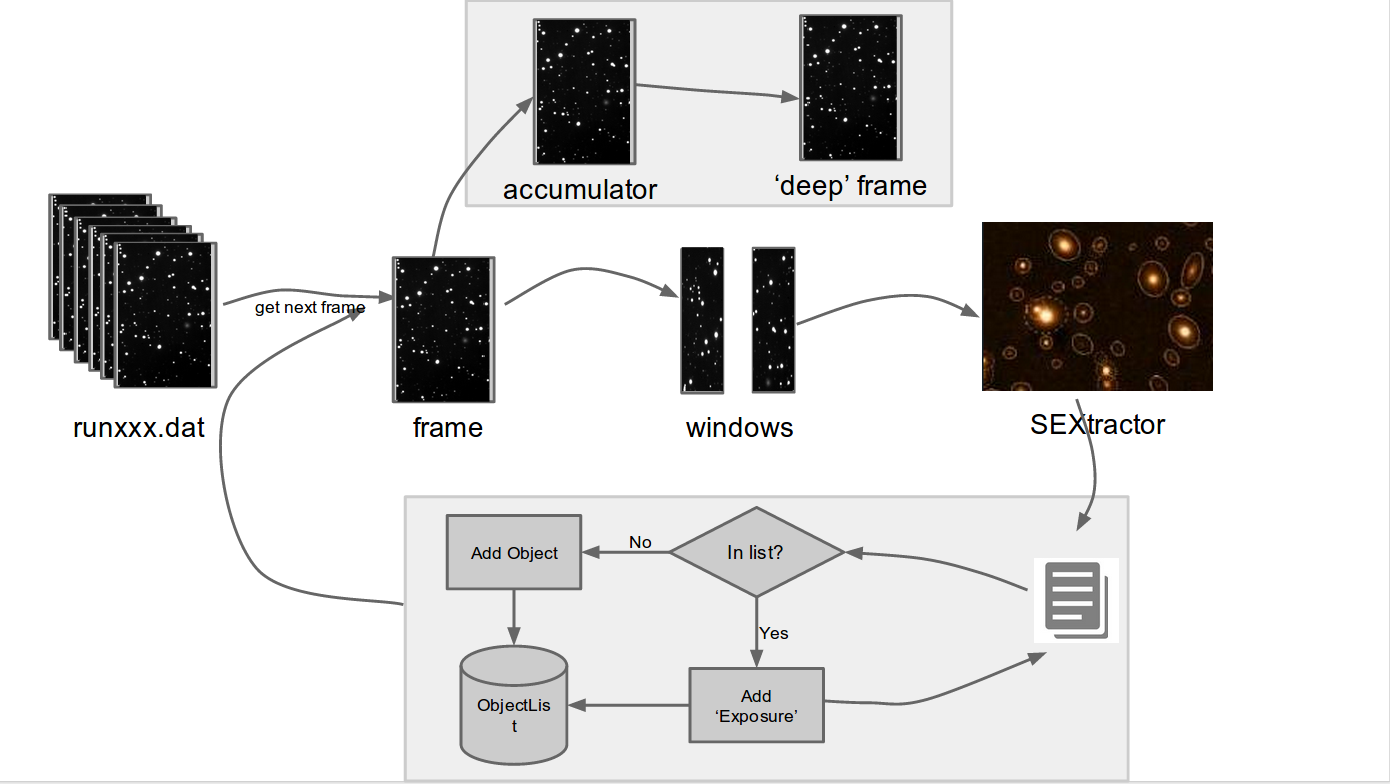
\includegraphics[width=130mm]{images/flowchart.png}
	\caption{Schematic of Stage 1 of the pipeline.}
	\label{flowchart}
\end{figure}


\begin{figure}[!h]
	\centering
	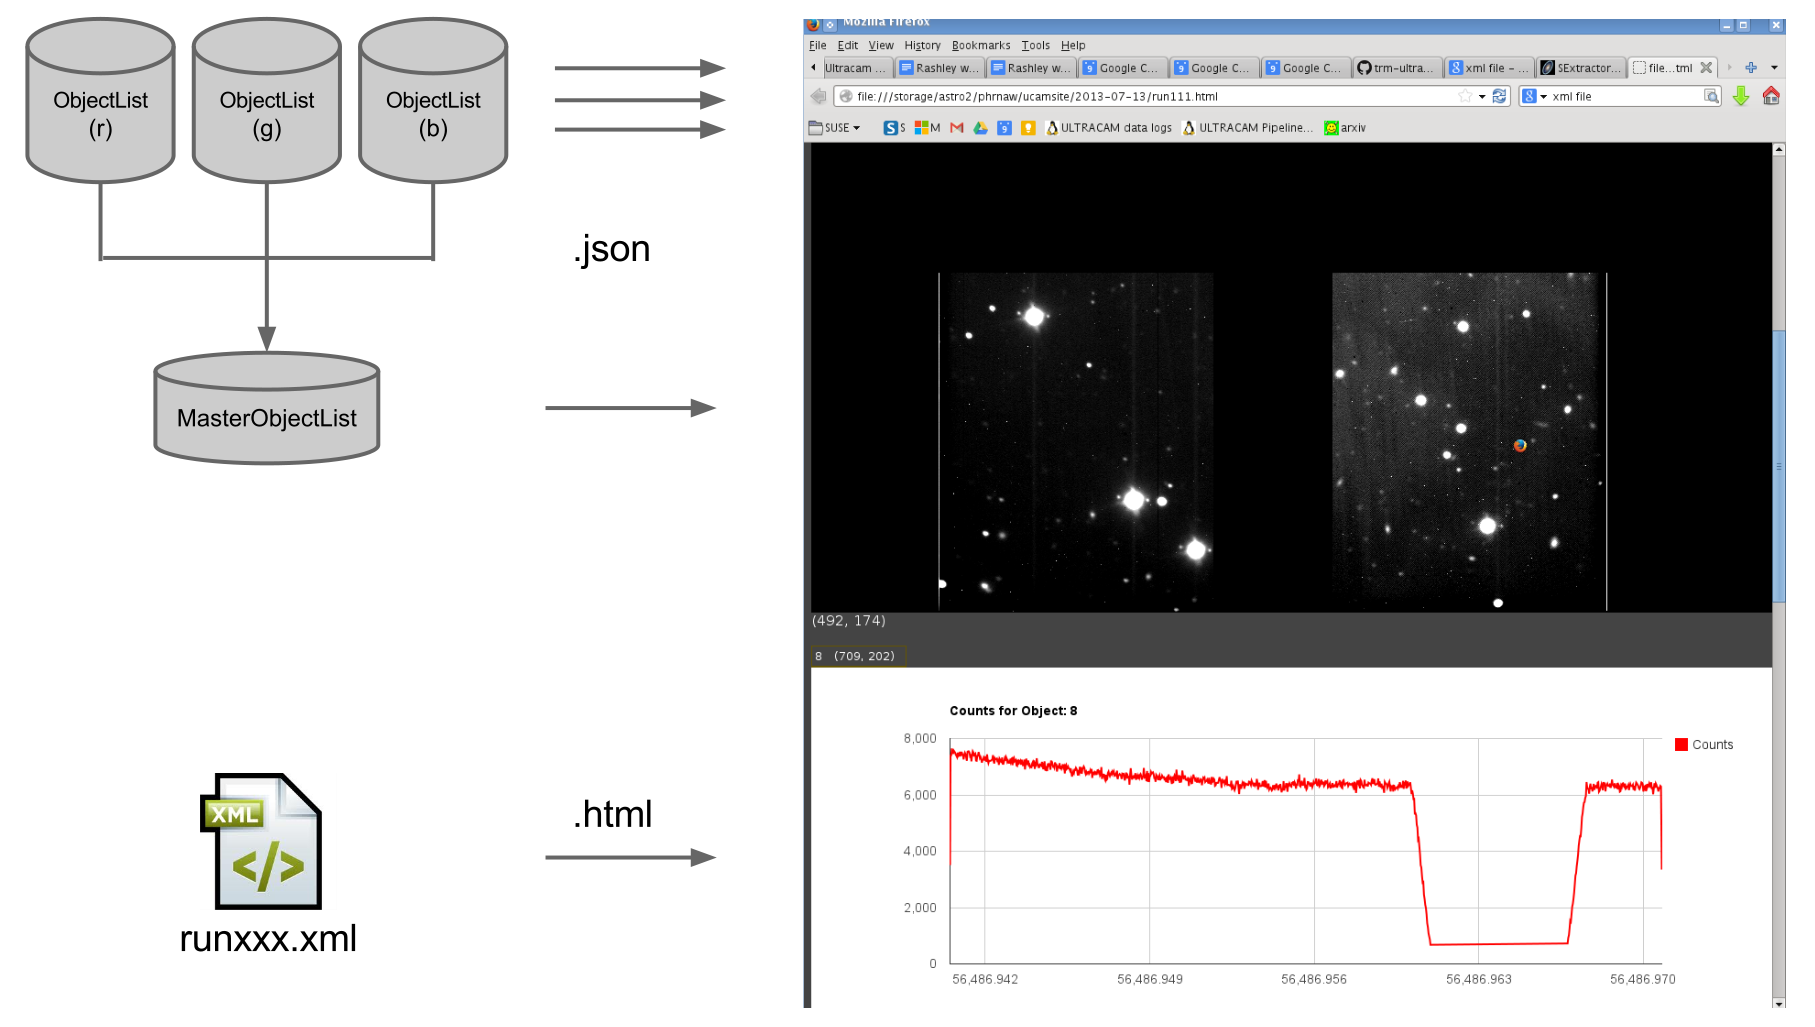
\includegraphics[width=130mm]{images/webpublish.png}
	\caption{Schematic of Stage 6 and 7 of the pipeline.}
	\label{webpublish}
\end{figure}

\subsubsection{Source extraction}
A popular software tool used for source extraction is SExtractor \cite{bertin}. SExtractor is able to process an image field and produce a catalog of sources in that field along with a measurement of the flux count of each object. The flux count is calculated after making efforts to account for the background in the field and then fitting a profile to the object. 

For each frame in the data run (which could consist of several to several thousand frames), we extract a bitmap of the image, which consists of a 2D pixel map with the CCD counts (or ADU) for each pixel, and pass this to SExtractor for source extraction. 

SExtractor performs two passes on this image. On the first pass it makes an estimate of the 'background signal' of the entire image. It does this by creating a mesh-grid of background readings for the whole image, applying a median clipping algorithm and then fitting a bicubic spline to interpolate between the mesh points. It then subtracts this background from the image. The size of the mesh grid is configurable and the pipeline allows the user to tweak this parameter if necessary, but it does \emph{not} adjust this parameter automatically. If small scale changes in the background are expected (for example, in runs like ??) then the mesh size should be reduced. The usual value that is used in the pipeline is a mesh grid size of \emph{64 pixels}.

On the second pass, SExtractor applies a convolution filter to the image. This step is intended to increase the detectability (enhance the Signal to Noise ratio) for target objects on the frame. The filter we are using by default for this automated pipeline is a simple 'circular' PSF defined by the 3x3 mask:
$
\begin{array}{ccc}
  1 & 2 & 1 \\
  2 & 4 & 2 \\
  1 & 1 & 1 \\
\end{array}  
$

\emph{Comment: Include a figure here showing a zoom of the image, pre and post filter. Doesn't really seem to make much difference.} 

SExtractor then applies thresholding to the background subtracted and filtered image. The threshold for detection is defined as the pixel's ADU value above the background (in units of the background's standard deviation). This threshold is configurable and can be modified before running the automated pipeline. The default value we have used for most of the pipeline processing so far is $3\sigma$. Decreasing this parameter can be used to increase the number of objects detected for any particular run but reducing it too much will cause the source extraction to produce too many spurious object detections. For example, setting this value to $1\sigma$ results in the source extraction identifying noise in the background as sources and this leads to the the automated pipeline being overloaded with new sources to process, grinding to halt as the number of potential objects climbs rapidly. At the moment, the automated pipeline is not able to automatically tune this parameter for each run, although this is something that should be considered for future iterations of the pipeline. Figure \ref{fig:tweakingthreshold} shows how reducing this threshold can increase the number of objects detected by the pipeline.

\begin{figure}
  \centering
  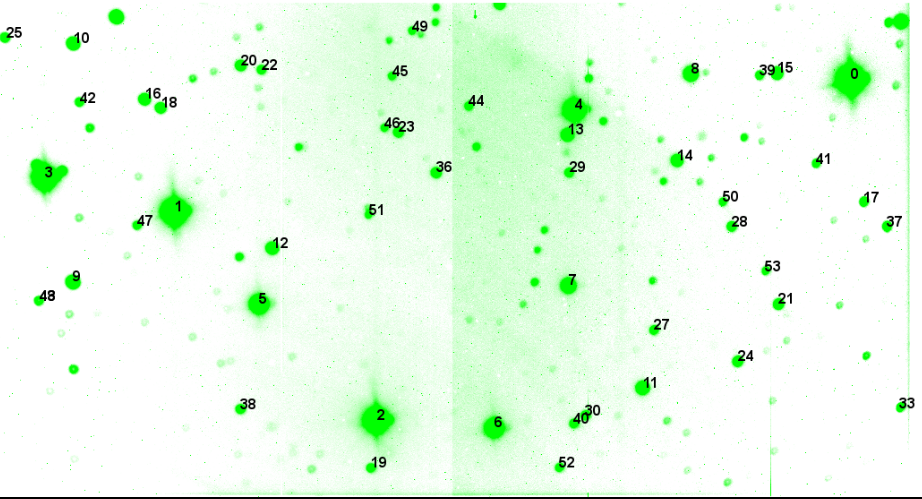
\includegraphics[width=.8\linewidth]{images/2012-09-03_g_default.png}
  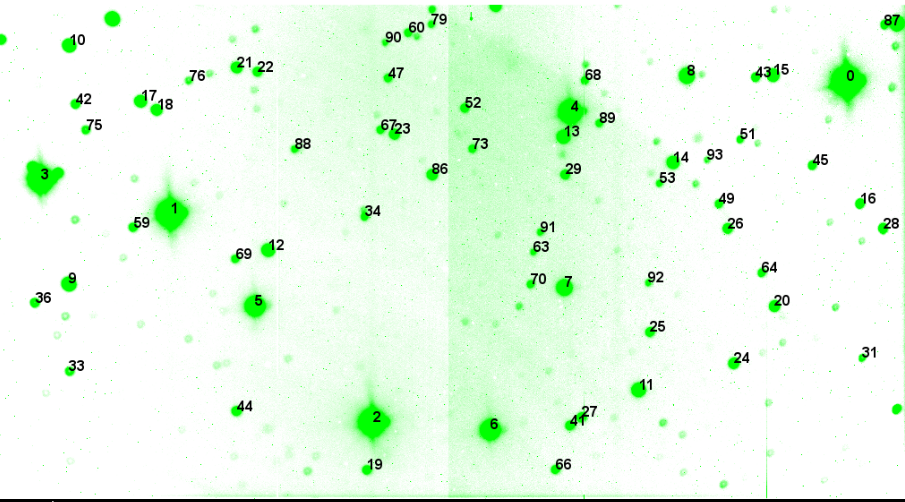
\includegraphics[width=.8\linewidth]{images/2012-09-03_g_15sigma.png}
  \caption{The effect of tweaking the DETECT\textunderscore THRESH parameter in SExtractor. The upper plot shows the objects detected in a run with the threshold set at $ 3\times \sigma_{background}$ [56 objects detected], while the lower plot was produced with DETECT\textunderscore THRESH set at $ 1.5\times \sigma_{background}$  [101 objects detected]. Note: setting it to 1.2 detected 149 objects, but took the pipeline 3x longer to run. }
\label{fig:tweakingthreshold}
\end{figure}

SExtractor then determines the pixel position of each object by calculating a weighted mean in the $x$ and $y$ dimensions. The weighting applied to each pixel is the pixel intensity (after background subtraction and filtering). If $I_{i}$ is the pixel intensity for pixel $i$ in the segmented collection of pixels, $S$ then:

$ X = \frac{\sum\limits_{i \in S} I_{i}x_{i}}{\sum\limits_{i \in S} I_i}$

$ Y = \frac{\sum\limits_{i \in S} I_{i}y_{i}}{\sum\limits_{i \in S} I_i}$

For each object that has been selected through the threshold criterion, the flux is then calculated. This is computed by one of 2 methods. 

\begin{enumerate}
  \item \emph{AUTO} Automatic aperture mode
SExtractor uses a routine inspired by Kron's ``first moment'' algorithm \cite{kron}. It defines an elliptical aperture that has an elongation $\epsilon$ and position angle $\theta$ defined by the second order moments of the object's light distribution. Across this ellipse, a first moment is computed $r_1 = \frac{\sum r I_r}{\sum{I_r}}$. The aperture is then scaled by user defined parameters to 2.5-3.5 times $r_1$. This is configurable by the user before the run, but usually does not require edits. 

  \item \emph{APER} Fixed aperture mode 
In this mode, the measurement of flux for the object is calculated by summing pixel intensity, $I_{x,y}$,  of all of the pixels that are within a pre-defined aperture radius centred on the x, y position as calculated above. 

$FLUX = \sum\limits_{x,y \in aperture}I_{x,y} $

The aperture radius is defined before the pipeline is run. This can therefore be adjusted manually. Due to the diversity of data in the ULTRACAM archive, there is no obvious single choice for this value. For example, some of the runs containing bright sources (ie magnitude 12 and brighter) found in the {SuperWASP}\footnote{\url{http://www.superwasp.org/}} and {HAT}\footnote{\url{http://hatnet.org/}} surveys use the telescope in a deliberately de-focused state, this is described in the introduction \ref{chap:introduction}. Aperture sizes for these runs need to be between 50 and 80 pixels. However, other runs with the telescope in focus and containing more crowded fields of objects need to be computed with far smaller aperture sizes of between 8 and 15 pixels. It is conceivable that the decision on which aperture size could be automated. A simple way to do this would be to perform a 2-pass approach. First use AUTO aperture mode to allow SExtractor to return a list of aperture sizes, then choose a fixed aperture size that represents the best choice for this run. This is something that will be considered for future iterations of the pipeline. 

\begin{figure}
  \centering
  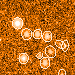
\includegraphics[width=50mm]{images/sex_apertures_auto_cropped.png}
  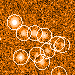
\includegraphics[width=50mm]{images/sex_apertures_fixed_cropped.png}
  \caption{AUTO vs FIXED apertures in SExtractor. The image on the left is the result of using the AUTO aperture setting in SExtractor. Note that apertures are elliptical. On the right is a FIXED aperture setting with the aperture diameter set (manually) to 15 pixels. The FIXED aperture is always circular.}
\label{fig:fixedautoapertures}
\end{figure}
\end{enumerate}

In order to facilitate the automatic running of the pipeline across the entire ULTRACAM data archive, the default setting for the flux measurement is the 'AUTO' aperture mode. This means that SExtractor uses the algorithm (described above) to determine the most appropriate aperture size for each object. After inspection of the output, runs that would benefit from fixed apertures can then be 're-computed' with a manual setting for the aperture size. 

The output from SExtractor is a FITS file that contains a catalog of all of the detected objects with measurements of their flux. Remember that, at this stage of the pipeline has no concept of 'state'. Each individual window of each frame in each channel (r, g, b) are treated separately by SExtractor and there is no tracking of objects from frame to frame or channel to channel. This task is undertaken by the automated pipeline software built for this project. 

\subsection{Object matching}
The automated pipeline needs to build up light curves for all of the objects and, in order to do so, it needs to keep track of these objects throughout the run (across frames and channels). The approach is to use the (x, y) coordinates of the objects returned by SExtractor as the key attribute for identifying an object that recurs from frame to frame. 

For each window sent to SExtractor, the pipeline performs the following steps:
\begin{enumerate}
  \item \emph{Read} the catalog file, containing (x, y) coordinates and fluxes for all objects in the window.
  \item \emph{Rank} all of the objects from brightest to faintest.
  \item \emph{Transform} the pixel coordinates from the reference frame of the individual window, to an overall frame, matching the size of the full CCD. 
  \item \emph{Match} all objects in the catalog. For each object in the list, check its proximity to any objects that have been identified on previous frames. The distance threshold for a match is configurable and the default is 10 pixels. If there is more than one match, the closest match wins. If there is no match, then this is a 'new' object and it is added it to the list of detected objects.  
\end{enumerate}

The algorithm is started with an empty list of objects. In the first frame, this list grows to include most of the objects we expect to detect in the run. However, the number of objects being tracked will slowly increase as the run is being processed. At this stage of the pipeline we do not remove any objects from our list. 

This approach will not cope with situations where the telescope may have been moved or disturbed during a run and there is a sudden 'step-jump' in the positions of all of the objects on the frame. This is sometimes referred to as a 'glitch'. If the 'glitch' results in a movement that is greater than the distance threshold (usually 10 pixels) then the pipeline will claim to have detected many new objects. In order to deal with glitches, we use a simple technique to determine the pixel shift $(\Delta x, \Delta y)$ for the each window, compared to the previous window. 

We create 2 dimensional map centred at zero, with all values set to zero. For each offset from every object in the current window to every object in the previous window $(\delta x, \delta_y)_i$ , we add '1' to the corresponding position in our image map at $(\delta x, \delta y)$. The resulting image 'histogram' will have a peak at a value of $(\delta_x, \delta y)_{max}$ which corresponds to the overall offset of the second window to the first. ie $(\Delta x, \Delta y) = (\delta_x, \delta y)_{max}$. We find the peak by first smoothing the image map and then fitting a quadratic around the maximum value and determining its value when the derivatives are zero in the $x$ and $y$ directions. We then apply this offset to our current window before looking for matches to objects in the previous window.

For each detected object in the window, we store: 
\begin{itemize}
  \item \emph{ID} A unique ID for this object that will persist across all frames for this object.
  \item For each frame in the run:
  \begin{itemize}
    \item \emph{Flux} The flux measurement for this object, as determined by SExtractor.
    \item \emph{Position} The pixel (x, y) position for this object, as determined by SExtractor, adjusted to the reference frame of the CCD. Note we do not include the small offset measured from frame-to-frame as determined be the image map procedure described above. 
    \item \emph{Flux radius} As measured by SExtractor, this is defined as the radius of the circle centred on the barycenter that encloses about half of the total flux. For a Gaussian profile, this is equal to $1/2$ the FWHM. 
  \end{itemize}
\end{itemize}

Before the pipeline attempts to match objects across each of the three channels (r, g, b), it performs a 'clean-up' of the data. It makes three passes of the object list performing the following filtering:

\begin{itemize}
  \item \emph{Cosmic ray} filtering. This step filters out any object that appears on only one frame in the run. 
  \item \emph{Low coverage filtering}. This step removes any objects that appear on fewer than a pre-defined percentage of frames. This value is configurable. The default is 20\%. This value should be set to '0' if we are looking for any kind of transient object in the run. 
  \item \emph{Single pixel filtering}. This step removes any object that has a \emph{Flux radius}, as measured by SExtractor, that is less than 1 pixel.
\end{itemize}

At this stage, the pipeline has produced three distinct object lists. One for each of the \emph{red}, \emph{green} and \emph{blue} channels. These lists are referred to as 'catalogs' as they now contain position and photometric information for each object detected in the run.  Now the pipeline attempts to cross-identify objects across all three catalogs. This is done based on the object's average position (x, y) in each channel and the minimum distance between it and it's corresponding location on the other channel. If there is an astrometric solution for each channel then this is used in favour of the pixel positions of the object as these solutions are likely to be far more accurate than the pixel positions. Unfortunately, for most of our runs, we do not have an astrometric solution and we have to revert to matching based on pixel distance. Astrometric solutions, and our difficulties with finding solutions, is discussed later in this chapter \ref{sect:astrometry}.

In the second pass,  we try to match an object across the three colours, the pixel position we use is the \emph{mean} pixel position of the object through the duration of the run. So we have three values to match $(\bar{x}, \bar{y})_{red}$, $(\bar{x}, \bar{y})_{green}$ and $(\bar{x}, \bar{y})_{blue}$. Since the red catalog (which is derived from the optical channel that is usually configured to use the the Sloan 'i' or 'r' filter) has the most number of objects detected, it is used to seed the 'master' catalog. In other words, the master catalog is initialised with all of the objects in the red catalog. For each object in the 'master' catalog, the pipeline consults the catalogs from the other two channels looking for a nearest match in distance (within a pre-defined threshold).

For each object in the green catalog indexed by the letter $i$, we calculate its distance from each object in the master catalog $Distance_j$. 

$D_j = \sqrt{(\bar{x}_{red, j}-\bar{x}_{green, i})^2 + (\bar{y}_{red, j}-\bar{y}_{green, i})^2})$ 

Then the matched master object for this green object is the one with the closest pixel distance $min(D_j)$. We merge these two objects together in the catalog, which contains one unique identifier (number) and the red and green photometry. If there is no match within the minimum distance threshold, then the object is treated as a 'new' object and added to the master catalog. It is possible that an object can be identified in the green channel, but not in the red. In this case, it is still added to the master catalog as a new object. This means that we have the capability of dealing with objects that have photometry in one or two colours, but not all three. 

The process is then repeated for the blue catalog. Again we match the blue coordinates to each object in the master catalog. First trying for a match of the blue coordinates to the red coordinates and then, if no match is found, we repeat looking for a match between the blue coordinates and the green coordinates.  

It is obvious that this is a very crude method of object matching. It is surprisingly robust for the majority of the ULTRACAM runs in the data archive. Many of the runs do not have crowded fields so there is little ambiguity in the object's positions. However, it can fail in a few situations. Since the red, green and blue channels do not have identical optical configurations, the images are not exactly aligned geometrically. The images in the r, g, b channels can differ from each other in terms of translation, rotation and distortion (across the image). This becomes particularly obvious for a full-frame image (using the full area of the CCD) and is most visible towards the edges. An example of this difference in the pixel locations from channel-to-channel can be seen in figures \ref{fig:nonoverlap} and \ref{fig:nonoverlapzoom}.

Yet another complication is caused by the change in these factors during the course of a long run, when the airmass of the target field undergoes a large change. The changes in the distortion due to the atmosphere varies in each channel. The change in the offset position from channel to channel can change by as much as ~4 pixels as the airmass changes from 1.0 to 1.2 and for larger airmass changes, the object will move by as much as 15 pixels in the blue channel relative to the red and green channels. 

\begin{figure}
  \centering
  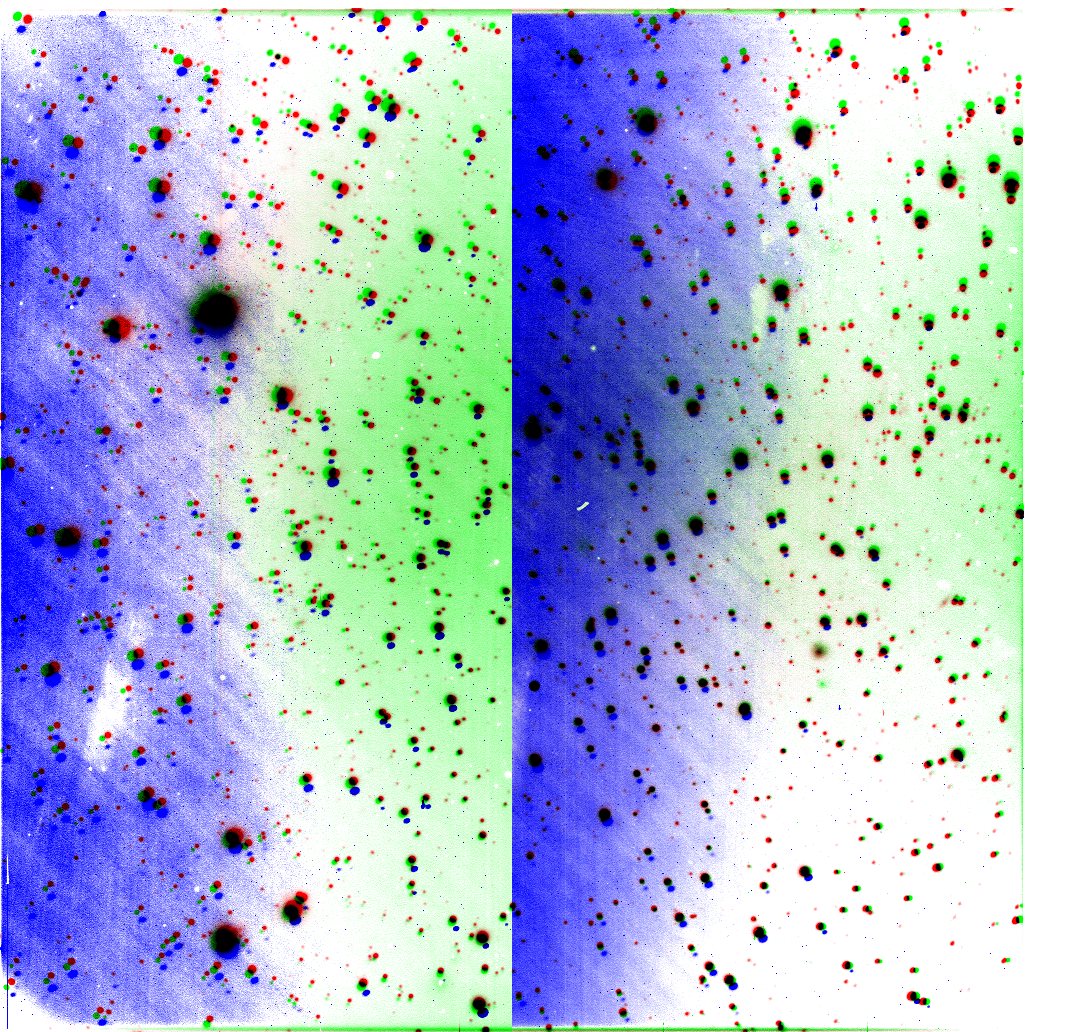
\includegraphics[width=100mm]{images/overlay_multiply.png}
  \caption{Images of the three channels overlaid (without any distortion correction applied). It is clear that the three channels do not have identical images. Translation, rotation and differential distortion are all visible. This makes matching of objects across the three channels difficult in some runs. }
\label{fig:nonoverlap}
\end{figure}



\begin{figure}
  \centering
  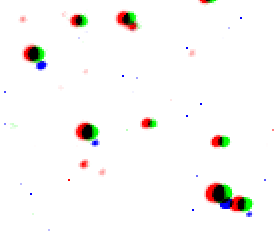
\includegraphics[width=50mm]{images/overlay_multiply_closeup.png}
  \caption{A close up of figure \ref{fig:nonoverlap} showing the bottom right hand corner. Note that the blue image is significantly translated from the red and green image. To make matters worse, this distortion is not constant through the duration of a single run and changes as the airmass of the target field changes.}
\label{fig:nonoverlapzoom}
\end{figure}

\begin{figure}
  \centering
  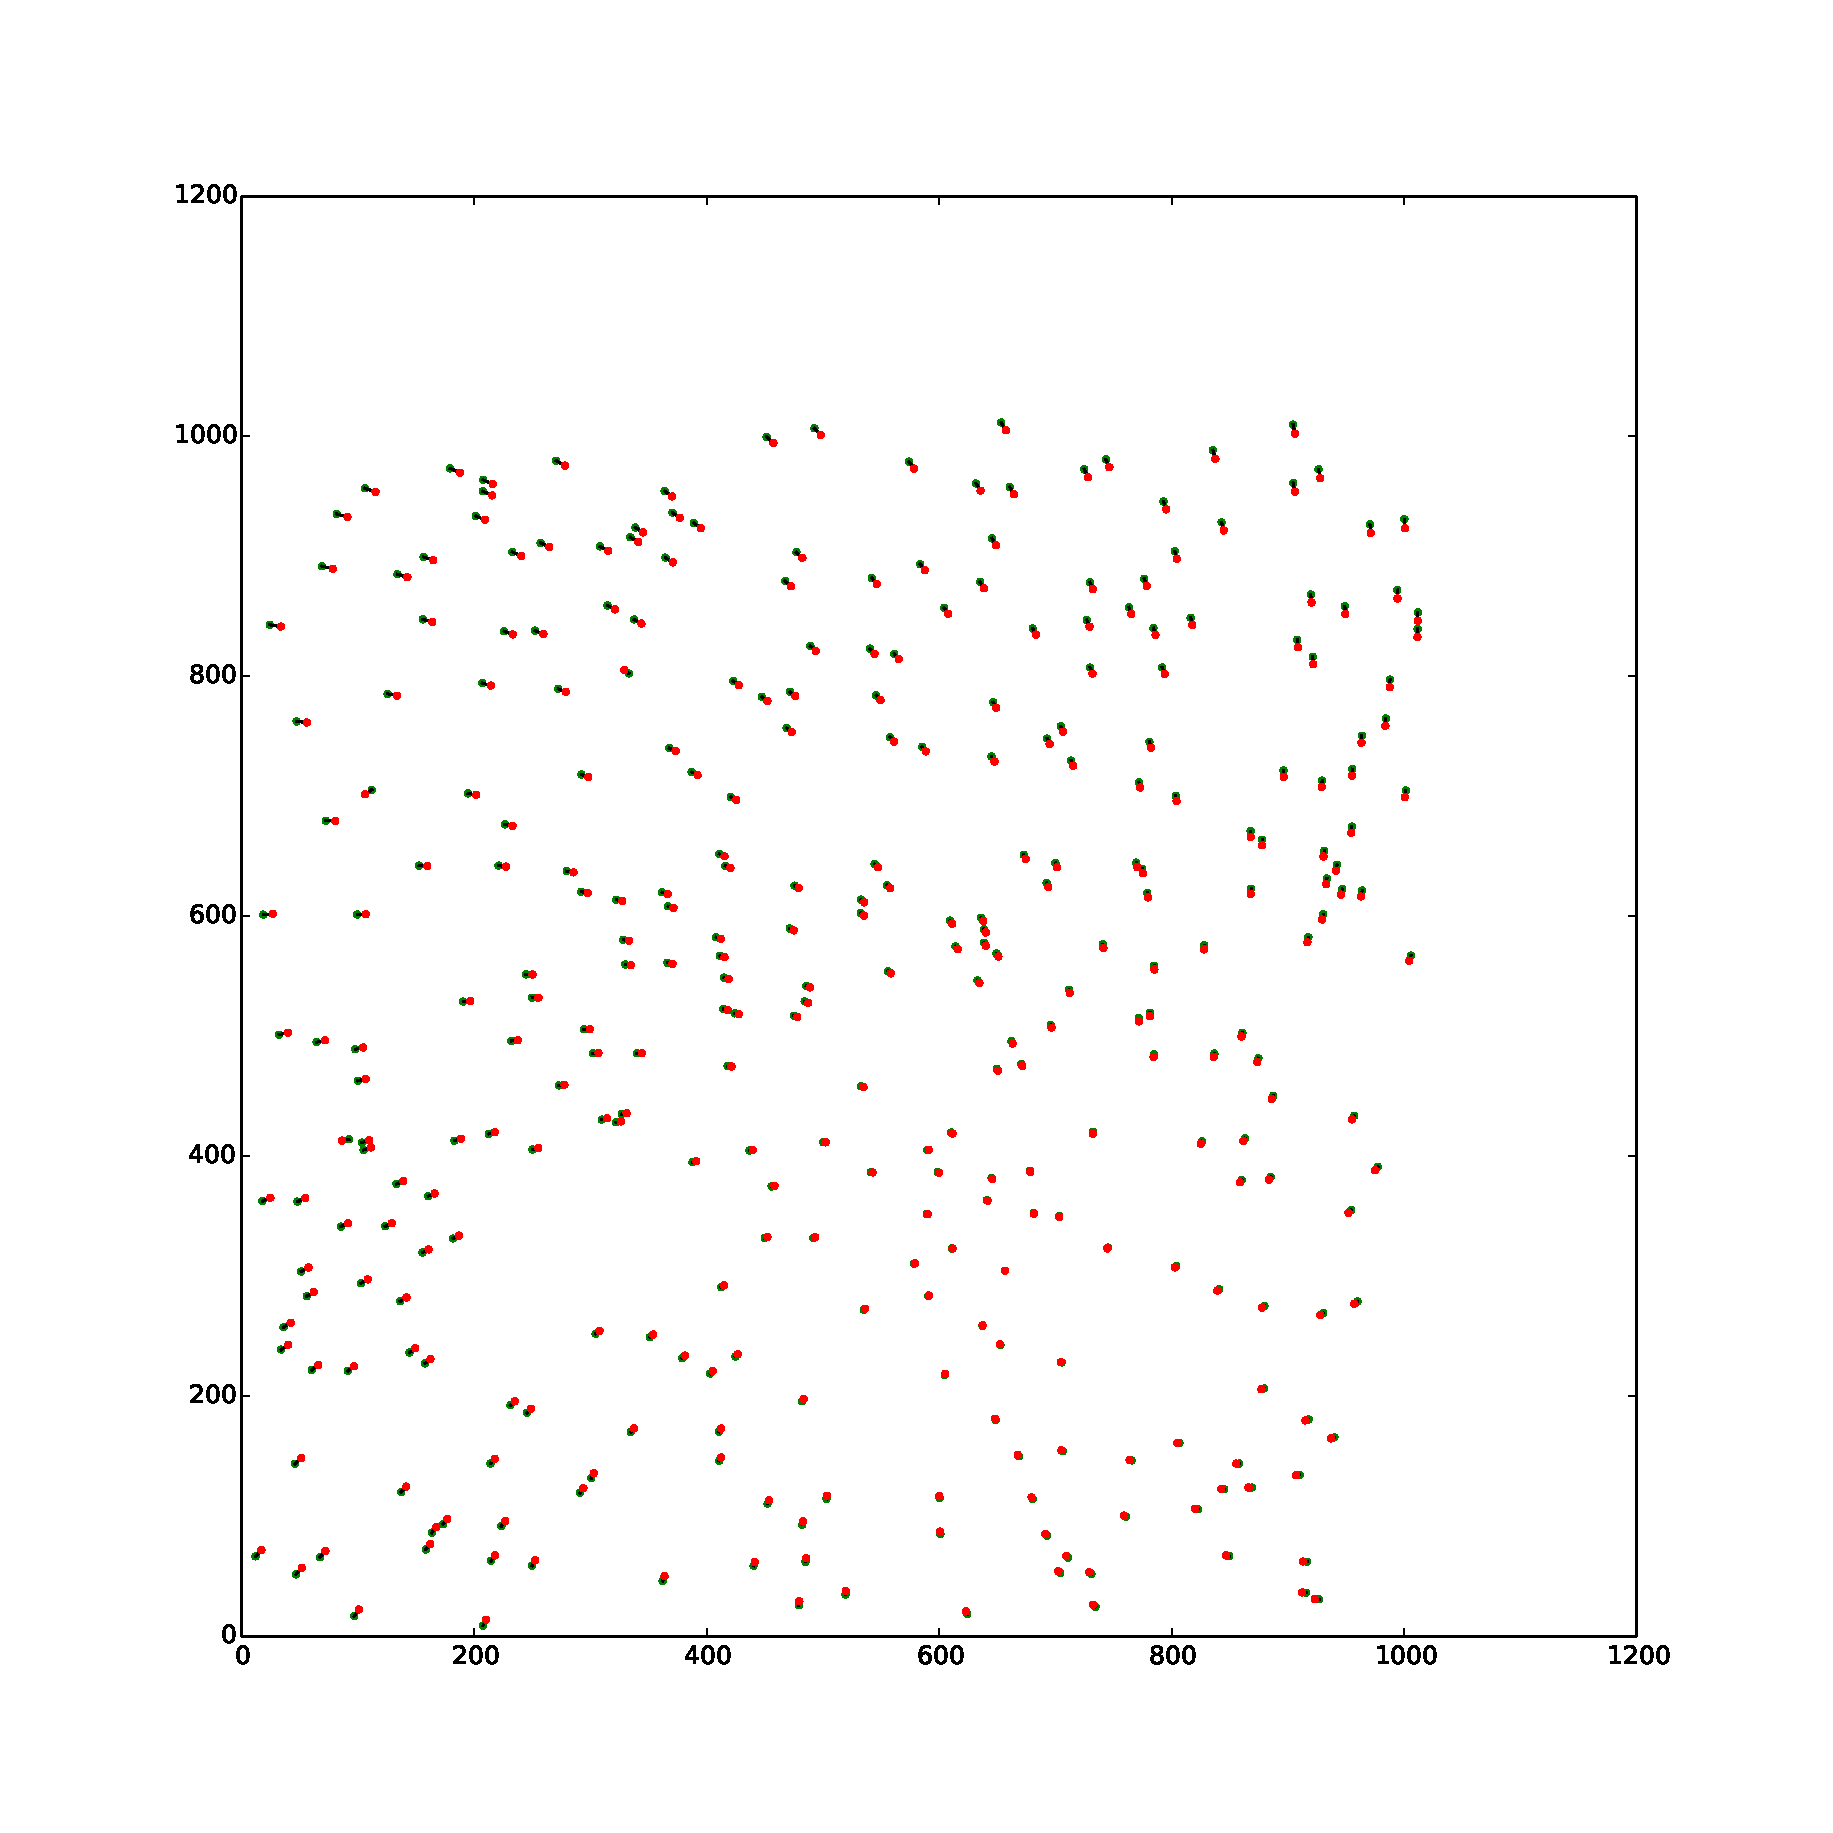
\includegraphics[width=60mm]{images/objectOffset_run010_g.eps}
  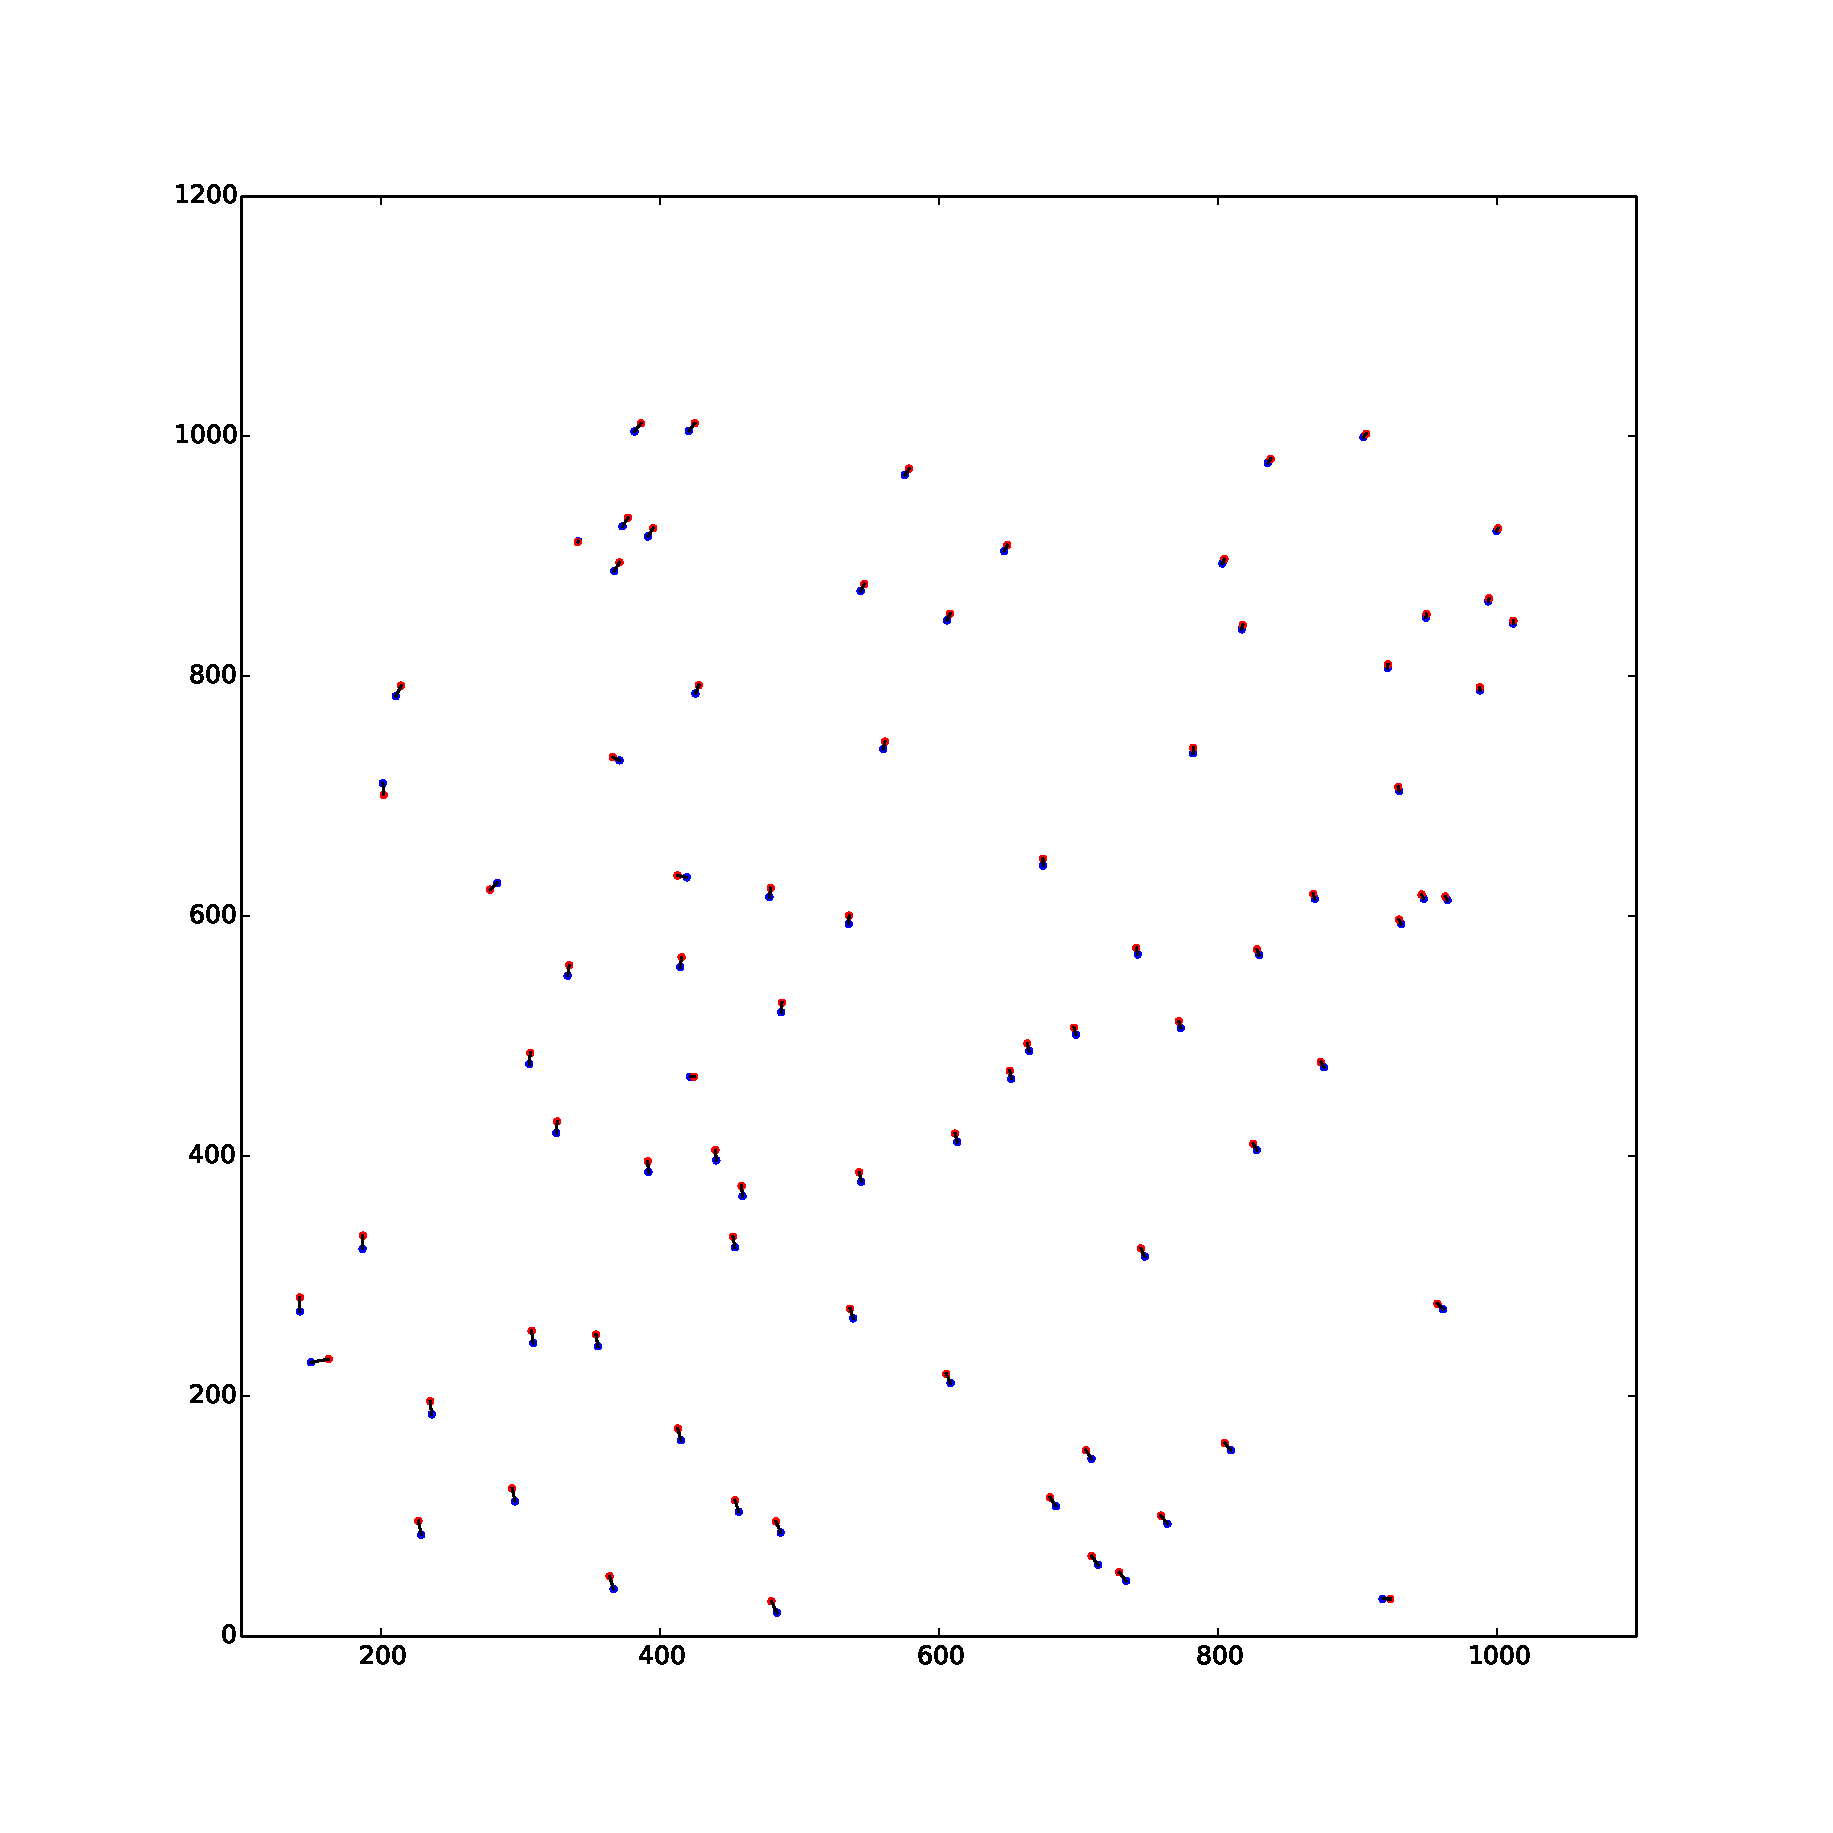
\includegraphics[width=60mm]{images/objectOffset_run010_b.eps}
  \caption{The difference in object positions between the 'red' channel and the 'green' channel (on the left) and the 'red' and 'blue' channel (on the right), for run: \emph{2013-07-21/run010} }
\label{fig:greenblueoffset}
\end{figure}



\begin{figure}
  \centering
  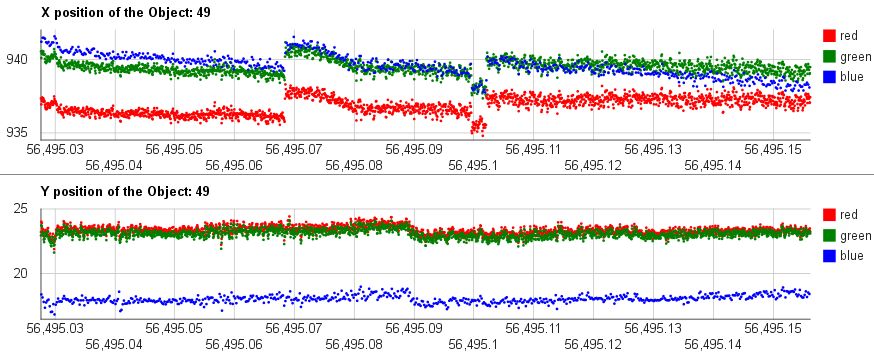
\includegraphics[width=140mm]{images/position_drift.png}
  \caption{Plot of the $(x, y)$ position of the object in the lower left corner of figure \ref{fig:nonoverlapzoom} showing how the position varies of the course of the run ~3 hours. During this time the airmass, $\sec z$, of the target field varies from 1.02 to 1.21. Note how the $x$ position of the object in the blue channel drifts from the $x$ position of the object in the red and green channels. The step changes in the object's position are caused by the observer making manual adjustments to the guiding at the telescope. }
\label{fig:positiondrift}
\end{figure}

\begin{figure}
  \centering
  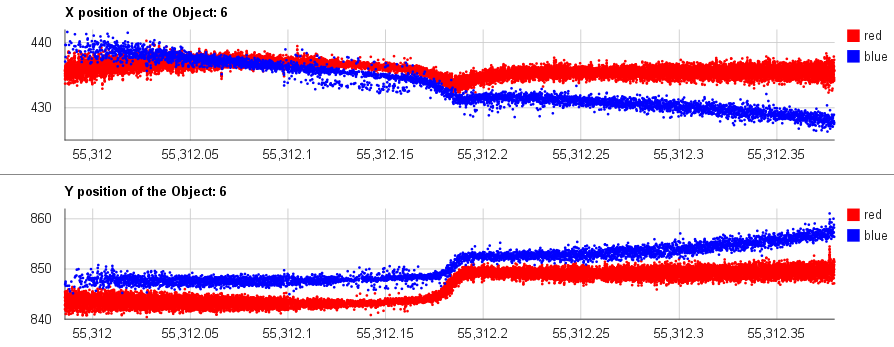
\includegraphics[width=140mm]{images/position_drift_longrun.png}
  \caption{Another plot showing the change in relative positions of a single object in different channels over the course of a long run. This data is taken from the longest run in the ULTRACAM data archive, the 9.5 hour long run \emph{2010-04-25/run020}. During this run, the airmass varies from a minimum of 1.0 (corresponding with the center of the plot), to a maximum of 1.99 (at the extreme left and right ends of the plot). The change in offset from the red to the blue channels is about most noticeable on the $x$ position, where the blue channel's offset moves by as much as 13 pixels. }
\label{fig:positiondriftlongrun}
\end{figure}

This trend is dealt with in the first stage of the pipeline by allowing the object to move gradually from frame-to-frame. It compensates by  constantly updating the object's position in each frame and using the new value as the comparison position when looking for matches in the next frame. It can deal with a general 'slow' migration in the object's position. So, in the first pass of the automated pipeline, when we are building the catalogs for each channel independently of each other, the have no problems with object matching. 

The process can fail when cross-matching across the different channels only if the \emph{average} position of the object is displaced by a large amount from channel to channel, or the field is crowded and there is more than one match for any particular set of objects. Fortunately, for many of the crowded fields, we can find an astrometric solution. In this case, we are no longer relying on pixel coordinates, but world coordinates to perform the match across the channels and these image distortions have been accounted for. 

\subsection{WCS solutions}\label{sect:astrometry}

After some ad-hoc tests using \emph{SCAMP \cite{scamp}} and \emph{Astrometry.net \cite{astrometry}} it seemed that the Astrometry.net software was more reliable at finding good WCS solutions to the fields. The software was downloaded to a local machine (including the extensive index files) and compiled. At the moment, this is now part of the pipeline but it does not consistently find WCS solutions for all of the fields. 

There are several challenges to finding a WCS solution for the fields.  These are:

\begin{itemize}
	\item \emph{Lack of pointing data}: ULTRACAM does not integrate with the pointing software of any of the telescopes and does not get pointing information automatically. We rely on the observer to enter a name of the candidate object for each run and then, when the data is archived, a \emph{SIMBAD} lookup is used. This gives us a world coordinate that is somewhere in the field, but it is not known which object (or pixel location) this applies to.  
	\item \emph{Field rotation}: Since ULTRACAM can be rotated about the optical axis to allow for optimal alignment of the objects, the field of view can be at any arbitrary angle of rotation, giving an extra degree of freedom to the matching task. 
	\item \emph{Windows}: Many ULTRACAM runs are configured to use only portions of the CCD area. You can see an example of this in Fig.  \ref{fig:V834Cen}. This means that there is an incomplete view of the sky for that field. When trying to match to existing indexes, there could be important, bright objects that are in the index file, but do not appear in the ULTRACAM field due to the masking caused by the windows.
	\item \emph{Sparse fields}: On uncrowded fields, we might only have 4-5 objects that can be used for field identification. 
	\item \emph{Very small windows}: Some runs, particularly ones in high cadence mode, use very small windows (eg 172x156 pixels) in order to decrease readout time. This means that our images (and input catalogs) might only contain two objects or so. This makes matching to a reference catalog impossible. 
	\item \emph{Choice of reference index by colour}: The Astrometry.net software uses 2MASS and Tycho-2 reference catalogs by default. These are based on infra-red and V magnitudes. This means that the blue channel (which is often using the SDSS u filter) might not match the reference indexes. Indeed, current tests often result in a match in red, a match in green but no match in blue. 
\end{itemize}

After the first stage of the automated pipeline we have three catalogs of objects for each of the channels (red, green and blue). These catalogs contain pixel coordinates and flux measurements for each frame in the run that the object has been identified. We produce a simplified catalog based on the mean pixel positions and mean flux for each object $(\bar{x_i}, \bar{y_i}, \bar{F_i})$. This catalog is then sorted in order of decreasing mean flux, $F$. The Astrometry.net package is given this input catalog and asked to find an solution astrometric solution for the field. 

Astrometry.net compares objects in its reference catalog to the catalog and pixel positions in the input. The matching algorithm is based on comparing the relative positions of quadruples of stars. The indexes are 'pre-built' and derived from the USNO-B survey, which contains $\sim10^9$ stars and Tycho-2 which has $\sim2.5\times10^6$ stars. 

In addition to providing Astrometry.net a catalog of objects to match, we also pass in the known location of the field that has been provided via a SIMBAD lookup of the coordinates of the target object as specified by the observer at the telescope. This gives us the world coordinates that are guaranteed \footnote{Provided that the telescope operator has correctly entered the target name, and the SIMBAD lookup has been successful.} to be somewhere within our field. We provide a limit to the coordinates of the solution as a maximum distance of 1 degree. We also provide upper and lower limits to the expected pixel scale of the solution. Providing these parameter saves computation time as it restricts Astrometry.net to a small region of the index and saves it from doing a comprehensive search. Considering that our field sizes are only a few arc minutes wide, specifying 1 degree as the search radius is probably overkill. A future task for this automated pipeline project will be to find the optimal values for this parameter.

If Astrometry.net can find a solution for our field, it generates a FITS format file containing the parameters defining the solution. These parameters consist of the position in right ascension and declination $(\alpha_{ref}, \delta_{ref})$ of a particular reference pixel in the image $(x_{ref}, y_{ref})$, plus 4 parameters that define a transformation matrix to move from pixel coordinates $(x, y)$ to world coordinates, $(\alpha, \delta)$. These values are labeled $CD1\_1$, $CD1\_2$, $CD2\_1$ and $CD2\_2$. The transformation from pixel coordinates to world coordinates is then given by: 

$\left(\begin{array}{c} \alpha \\ \delta \end{array} \right) = \left(\begin{array}{c} \alpha_{ref} \\ \delta_{ref} \end{array} \right) + 
\left(\begin{array}{cc}  CD1\_1 & CD1\_2 \\ CD2\_1  & CD2\_2 \\ \end{array}\right) 
\left(\begin{array}{c} x' \\ y' \end{array} \right)$

Where $(x', y')$ are the pixel offsets to the reference pixel $(x_{ref}, y_{ref})$.

These values are saved to the web repository as a JSON object, ready to be loaded when the web browser accesses the page. 

These 4 values define a scale transformation and a rotation from pixel to world coordinates. They do \emph{not} take into account distortion across the image. In order to encapsulate this distortion, Astrometry.net also provides Simple Imaging Polynomial (SIP) correction parameters \cite{sippolynomial}. In this project, we use a SIP polynomial of the 3rd order to account for distortion across the ULTRACAM field. Figure \ref{fig:sippolynomial} shows the SIP polynomial corrections applied to the positions of each object identified in the run \emph{2013-07-21/run010}. The correcting factors provided by this polynomial are generally very small, providing a corrections of a few thousandths of a pixel in most cases. 

\begin{figure}
  \centering
  \includegraphics[width=60mm]{images/SIP_run010_r.eps}
  
  \includegraphics[width=60mm]{images/SIP_run010_g.eps}
  
  \includegraphics[width=60mm]{images/SIP_run010_b.eps}

\caption{An indication of the distortion present in the field for the 'red', 'green' and 'blue' channels of ULTRACAM. The background bitmap shows the deep image of the field. The vectors leading away from the objects were generated by calculating the 'World' coordinates (WCS) for the object's position (without the SIP corrections) and the reverting those WCS coordinates back to pixel coordinates (using the SIP corrections). The displacements have been exaggerated by a factor of $10^7$.}
\label{fig:sipfit}
\end{figure}


\subsection{Web publishing}
A key aim for this project is to make all of the ULTRACAM's data archive available for browsing and accessible to a wider and more geo-graphically dispersed audience. The obvious approach is to make the output of the project available through a web enabled interface. From the outset of the project, all efforts have been focused on ensuring that the resulting data is all accessible through an easy-to-use web interface. 

HTML, CSS and JavaScript are three core technologies driving the development of the dynamic, interactive and flexible applications we are becoming accustomed to on the web these days. We chose these three technologies to present the ULTRACAM archive. The result of this is that this archive is immediately available to anyone with a modern web browser and working on any type of computer (desktop, laptop or tablet). There are some high demands on memory, so it is not recommended that the archive is browsed using a mobile phone, although, in theory, there is no functionality that restricts use on such a device (just the memory constraints). 

\emph{HTML} provides the underlying structure of a modern webpage. It is a semantic markup language, meaning that its purpose is to inform the browser on the document's structure. Despite the habit of many people who dabble at making web pages, HTML is \emph{not} meant to be used to alter the presentation of content. \emph{CSS (or Cascading Style Sheets)} is the layer that is meant to inform the browser on how the presentation of each element on the page should look. For example, it might define the fonts or colours for each particular element (or set of
 elements), like headings, paragraphs, etc. \emph{Javascript} provides the interactive portion of the page, allowing the user to trigger actions when a mouse is
 clicked or a new object is loaded. It can be used to manipulate the structure of the existing page. It also provides the mechanism for mathematical computation.

Another way of stating this is to say that HTML provides the Semantic structure, CSS the Presentation layer and JavaScript the Programmatic environment. This is also described as the classic "Model-View-Controller" approach used in many development paradigms in the field of Computer Science.

The final stage in the ULTRACAM automated pipeline produces a set of files that are available to a web browser. These files are hosted on a web server that is operated by the University of Warwick CSC team. The pipeline prepares that files and then writes them to the appropriate location in the University's local storage. As soon as the pipeline has finished running, the web pages can be viewed globally. 

Web applications like this, are often refered to as 'client-server' applications, meaning that the application consist of two parts, one running on the client (web browser) of the end-user and the other part running on the server of the institution hosting the application. Obviously, there is a one-to-many relationship between clients and server. There is usually only one server involved, but many clients can connect to that server and interact individually with the application. When writing this pipeline we had to make a decision on how much of the functionality we should place on the server versus the client. There were two main (competing) factors to consider:

\begin{itemize}
  \item Complexity of the application: Writing an application that has complex components on both the server-side and the client-side, increases the difficulty in launching and maintaining the application. We need to install and configure a web server that is able to run code locally and that also needs access to local data sources, such as databases. If we structure our application such this is only relies on the web server to server static files, then the management of the server-side portion is trivial. If, on the other hand, we decide to split the application code to run on both the client and the server, then we need code on both components that will handle the interaction between the the two and data sessions need coordination. Also, the connection between the two can add some latency (time-lag) to the interactions. 

  \item Browser memory constraints: Loading all of the data required to display the results of one of the ULTRACAM runs can be quite demanding on the browser. For some runs there are several hundred objects each with several hundred exposures. This can result in a JSON file for the object data that is > 1 MByte in size. All of this has to be loaded into the browser's memory. If the user is working on a tablet or an older desktop PC or laptop, then this can cause memory issues. Some long runs with extremely high cadences have very few objects, but 100s of thousands of exposures for each and these will also tax the memory on the browser. That said, it is true that for the vast majority of the runs, the memory load on the browser, although significant, is not a problem.   
\end{itemize}

In order to aid rapid development of this project, we decided to opt for a purely client-side code implementation, leaving the web server to serve only static files. This is working adequately in te
rms of meeting the needs and scope of the project, but it is clear that, for future iterations of this pipeline we should carefully consider moving to an application model that relies more heavily o
n the server to manipulate, store and serve data. We cannot place any more load on the client. 

We chose JSON (JavaScript Object Notation) \footnote{\url{http://json.org/}} as the format to store our data as this meant that it could be easily loaded by the Javascript code running in the browser. JavaScript has several built-in methods to load and parse a JSON object. JSON is a flexible, open format that allows a hierarchical structure to be defined for each object stored. It is also designed to be human-readable, meaning that it is possible to open in a text editor and check to contents. The problem with this format is that it is in 'plain text' and uncompressed. Also the format includes the structure of each object, leading to some amount of redundancy in the file (repeating of labels, etc). While it is true that JSON is inefficient in many ways, it is a useful format to use thanks to its flexibility and the ease with which the developer can check and debug the data. 

The core `visible product' of the project is a website that allows a user to browse all of the data in the ULTRACAM archive. The key features of this website are:

\begin{itemize}
	\item A catalog of runs organised by calendar date, containing \emph{thumbnail images} of the fields.
	\item For each run, a web page that shows the user:
	\begin{itemize}
		\item the \emph{deep images} of the field in each of the three channels (r, g, b).
		\item the \emph{light-curves} of each object as the user clicks on the object with the mouse. 
		\item the sky coordinates of each object and the mouse position, provided that a correct astrometric solution has been found for the run. 
		\item the light curve for the object that is currently being used as the 'comparison' object. 
	\end{itemize}
	\item light-curves should be plotted as absolute measured flux or a \emph{relative flux} compared to some other objects in the field. 
	\item the web page should also allow the user to \emph{export} the data to a standard format.
	
\end{itemize}
See Fig. \ref{browser} for an example of the web-page. 

\begin{figure}[!h]
	\centering
	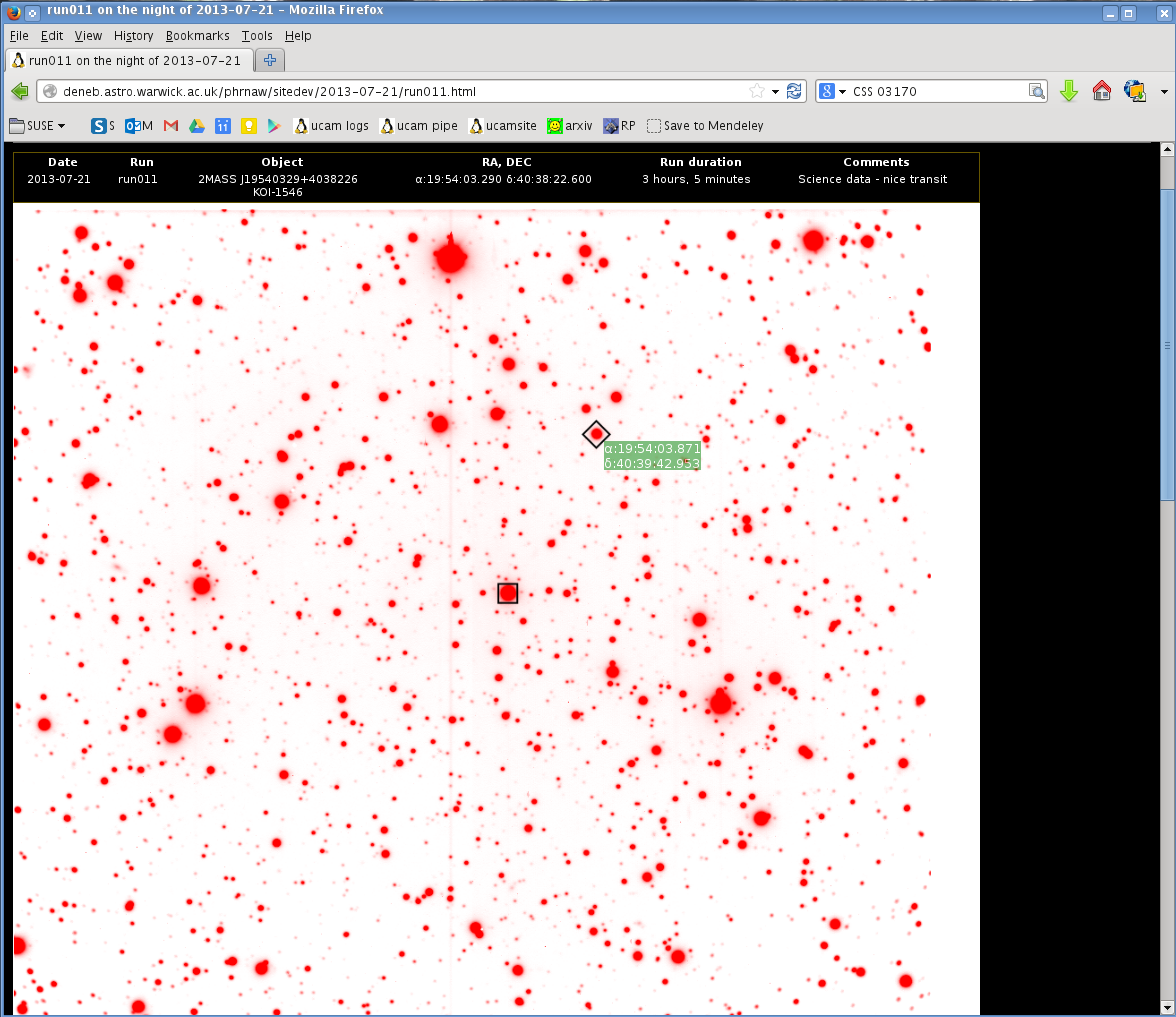
\includegraphics[width=90mm]{images/website1.png}
	\caption{Preview of the webpage.}
	\label{browser}
\end{figure}

